\section{Experiments and Results}
This chapter describes the evaluation methodology and outlines the metrics and figures that we used to quantify the performance of our learned policies on both single-quadrotor and multi-quadrotor cable-suspended payload transport tasks.













    
    




    



    
    




\subsection{Baseline Comparison}

We benchmark the decentralized \gls{rl} policy against the baseline of \cite{wahba_kinodynamic_2024}, which models each cable as a rigid rod and relies on centralized trajectory optimization with an online tracker. This limits responsiveness to cable swing, mode changes, disturbances, and payload variations. In the two quadrotors with payload scenario the payload begins at \((0,0,1.5)\,\mathrm{m}\) and the vehicles are randomized around it, and both methods pursue the same goal. We evaluate in simulation to enable statistical analysis and tightly controlled initial conditions. Each method is executed for \(N=1000\) trials with randomized payload states and vehicle poses. To favor the baseline we precompute a higher order straight line polynomial trajectory from start to target and have the baseline track it.

Our learned policy achieves \(797\) successful recoveries out of \(1000\) trials \(\bigl(79.7\,\%\bigr)\) with a mean speed of 0.58~m/s. The baseline achieves \(435\) successful recoveries out of \(1000\) trials \(\bigl(43.5\,\%\bigr)\) with a mean speed of 0.27~m/s. Given identical start and goal distance, the higher mean speed together with the higher recovery rate indicates shorter and more reliable recoveries for our method. Qualitatively our policy damps swing quickly and follows a nearly straight approach, whereas the baseline often dips and then spirals, which is consistent with its rigid rod cable model.

\begin{figure}[]
    \centering
    \includegraphics[width=\textwidth]{baseline_recovery.png}
    \caption[]{Example recovery trajectories from eight harsh initializations. Top: XY; bottom: XZ. Our Method with visualized payload velocity (colormap) vs.\ baseline (thin gray).}
    \label{fig:baseline_recovery}
\end{figure}
\subsection{Generalization}
\begin{figure}[ht]
    \centering
    
    \includegraphics[width=\textwidth]{generalization.pdf}
    \caption[Policy Generalization]{Evaluation of the learned policy's generalization capabilities in the two quadrotors with payload scenario. Each datapoint represents the percentage of successfully recovered runs out of 1000 runs in an environment that only differs in the specific value adjusted. The policy is trained on a 0.3~m cable length and a payload mass of 0.01~kg.}
    \label{fig:generalization}
\end{figure}

 We assess generalization in the two quadrotor payload task by sweeping cable length ($L$), payload mass, observation noise scale ($\sigma_\text{obs}$), and initialization seed. Success is the fraction of runs that recover within 10\,s. As shown in Fig.~\ref{fig:generalization}: (i) Cable length: shorter cables sharply reduce success (increased collision risk). Moderate increases above 0.3\,m improve success, while very long cables ($>1$\,m) degrade performance as the payload becomes harder to stabilize. (ii) Payload mass: performance is robust across a broad range; lighter payloads show a slight drop, and heavier payloads reduce success more noticeably. (iii) Observation noise: the policy is tolerant up to a scale of about $1$, with a steep decline beyond that. (iv) Seeds: results are largely insensitive to initialization, consistent with training across 16k parallel environments. Overall, the policy generalizes well to unseen dynamics without explicit domain randomization, which indicates strong robustness.
\subsection{Scalability}
Our framework scales from a single vehicle to larger teams. We evaluate $Q\in\{1,2,3,6\}$ on two tasks in simulation, harsh recovery from initialization as shown in Fig.~\ref{fig:env-reset} to a fixed target and tracking of a figure eight reference trajectory as shown in Fig.~\ref{fig:scale-8}. Each setting uses $1000$ trials with a policy trained for the given team size.

For $Q{=}1$ the system stabilizes from up to $1\,\mathrm{m}$ displacement in about $2\,\mathrm{s}$ with a $99\%$ success rate and tracks the figure eight with a small phase lag.  
For $Q{=}2$ recovery succeeds in $81\%$ of trials with a similar settling time and failures occur mainly at the beginning under extreme initial states that cause collisions.  
For $Q{=}3$ with a $20\,\mathrm{g}$ payload, the team reaches $60\%$ recovery success and shows coordinated load sharing.  
For $Q{=}6$ with a $40\,\mathrm{g}$ payload, most runs terminate early, which exposes a coordination limit.

The main bottleneck seems to be permutation sensitivity in peer observations. Sorting peers by distance or adding attention-based aggregation and a richer payload representation are promising next steps.
\begin{figure}[t!]
    \centering
    
    \includegraphics[width=\textwidth]{fig8_scale.png}
    \caption{Figure eight trajectory tracking in simulation with one, two, and three quadrotors carrying a payload. Each column shows five runs starting at harsh initial conditions. Left $Q{=}1$ quadrotors, middle $Q{=}2$, right $Q{=}3$. The solid colormap curve is the payload trajectory with color indicating speed magnitude. Dotted curves are vehicle trajectories.}
    \label{fig:scale-8}
\end{figure}
\subsection{Sim-to-Real Transfer}

We deploy the learned decentralized policy on Crazyflie quadrotors by exporting it to TFLite and compiling with STM32Cube.AI for the STM32F405. On each quadrotor, an identical copy of the policy runs at \(250\,\text{Hz}\). Each robot builds its own observation from the onboard \gls{ekf} state (position, velocity, attitude, and rates) together with the measured positions of the payload and teammates from motion capture, mapped to the policy input. There is no centralized coordinator and no cross vehicle inference; the control loop runs fully onboard. The policy outputs individual motor commands that are converted to PWM and sent directly to the motors.

In flight tests, we observe robust autonomous takeoff, strong disturbance rejection, and stable flight in wind for a single quadrotor with and without payload, and for two quadrotors carrying a payload. In the wind trials, the measured average wind speed at the midpoint of the figure eight trajectory is 3.5~m/s. Figure~\ref{fig:overview} illustrates takeoff and disturbance rejection behavior with two quads and a $10\,\mathrm{g}$ payload. Figure~\ref{fig:fig8} shows two robots maintaining a figure eight payload trajectory even in a windy condition.


\begin{figure}[t!]
    \centering
    
    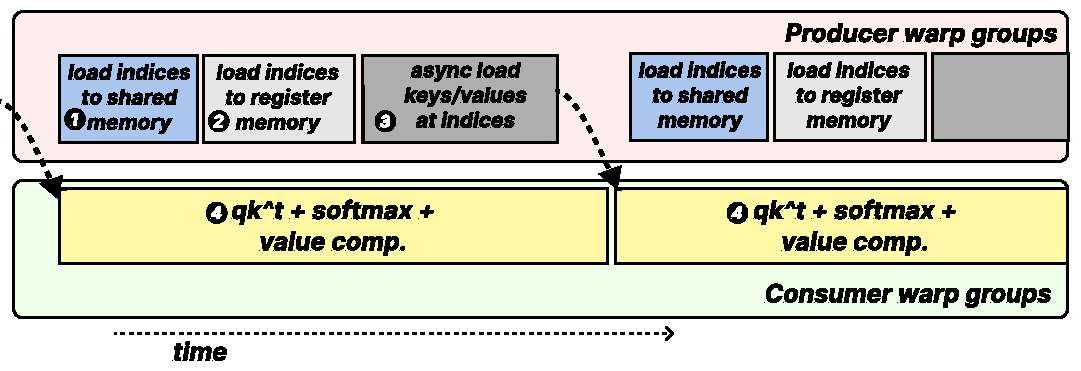
\includegraphics[width=\textwidth]{fig8.png}
    \caption[]{Two quadrotors with \gls{rl} policy cooperating to ensure the payload stays on a figure eight trajectory with and without wind disturbance.}
    \label{fig:fig8}
\end{figure}
